% Úvod
%---------------------------------------------------------------------------
\chapter{Úvod}
Tradičné redakčné systémy pre správu obsahu sú obvykle zostavené z~dvoch hlavných súčastí -- administračného a verejného webového rozhrania. Administračné rozhranie slúži pre vytváranie a úpravu obsahu, webové na jeho nasledné zobrazenie. Webové rozhranie je obvykle jednotné pre všetky platformy a zariadenia na ktorých je využívané, tzn. že jeho používanie je často neoptimálne. Pre tento dôvod sa začali využívať systémy bez webového rozhrania disponujúce klasickým administračným rozhraním a otvoreným aplikačným rozhraním (API\footnote{API -- Application programming interface}), umožnujúcim získavanie obsahu na požadované platformy. Tento obsah je následne možné optimalizovať individuálne podľa potreby. Súčasné riešenia redakčných systémom s~otvoreným rozhraním sú často robustné systémy, ktoré však vyžadujú komplexnú konfiguráciu predtým ako ich je možné začať využívať. Niektoré takéto systémy vyžadujú aj vlastnú infraštruktúru pre ich nasadenie. Tieto skutočnosti otvárajú priestor pre redakčný systém, ktorý by pomohol vyriešiť tieto prekážky. Takýto systém je cieľom tejto práce.

Navrhovaný systém poskytuje možnosť správy obsahu bez nutnosti úvodnej konfigurácie a infraštruktúry. Obsah je možné spravovať pomocou užívateľského rozhrania v~aplikácii Slack alebo webového rozhrania. Plnú funkcionalitu však užívateľ môže využiť bez nutnosti používania webového rozhrania.

\subsection*{Obsah kapitol}
Prvá kapitola, \nameref{chapter:theory}, sa skladá zo~štyroch sekcií venovaným postupne existujúcim riešeniam podobným tejto práci, vývoji serverových aplikácii, klientských aplikácii a~špecifikácii GraphQL.

% TODO: Add introduction to document's structure.

% Teoretická časť
%---------------------------------------------------------------------------
\chapter{Teoretická časť}
\label{chapter:theory}
Správa obsahu a jeho doručenie konzumentom. Táto kapitola popisuje základné princípy, techniky a technológie, ktoré sú nutné pre zostavenie a pochopenie princípu fungovania tejto práce. V~prvej sekcií \ref{section:headless} sú bližšie priblízené redakčné systémy s~otvoreným aplikačným rozhraním, v~druhej sekcií \ref{section:server_dev} vývoj serverových aplikácií, tretia sekcia \ref{section:client_dev} popisuje vývoj klientských aplikácii a posledná sekcia \ref{section:graphql} vysveluje špecifikáciu GraphQL.

\section{Redakčné systémy s~otvoreným aplikačným rozhraním}
\label{section:headless}
Redakčné systémy disponujúce iba skrytou administračnou časťou a verejným aplikačným rozhraním sú typicky nazývané \textbf{headless}\footnote{headless -- ang. bez hlavy (bez webového rozhrania)} redakčné systémy. Tieto riešenia štandardne disponujú rozhraním REST\footnote{REST -- Representational State Transfer} alebo GraphQL, ktoré implementuje aj táto práca. Headless redakčný systém nerieši zobrazenie samotného obsahu. Jediný spôsob ako obsah získať je využiť niektoré z~dostupných rozhraní poskytované konkrétnym riešením. Výhodou oproti tradičným redakčným systémom je možnosť získané dáta optimalizovane zobraziť na rôznych zariadeniach. 

\begin{figure}[h]
	\centering
	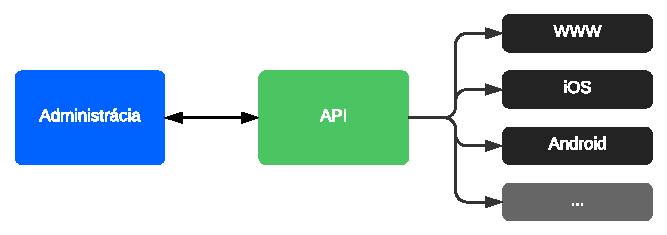
\includegraphics{obrazky-figures/headless_cms_graph.pdf}
	\caption{Ilustračná schéma generického headless redakčného systému.}
\end{figure}

\noindent Členenie obsahu v~takýchto redakčných systémoch je typicky v~dvoch vrstvách -- kategórie a obsahové typy (komponenty). Kategórie sú zoznamy združujúce jednotlivé komponenty, môžu byť homogénne (všetky prvky zoznamu sú jednoho typu) alebo heterogénne (prvky zoznamu sú typicky iných typov). Komponenty sú atomickými prvkami headless redakčných systémov. Môžu nadobúdať rôznych typov, ktoré určujú ich vnútornú dátovú štruktúru. Typický príklad často používaných typov komponentov sú napríklad \texttt{prostý text} alebo \texttt{odkaz}. Niektoré headless redakčné systémy umožňujú vytvárať aj vlastné typy komponentov a tak si prospôsobiť dáta vlastným špecifickým potrebám.

\subsection{Strapi}
Najpopulárnejší Headless redakčný systém. Disponuje administračným panelom zostaveným namieru, REST aj GraphQL rozhraním, systémom uživateľských práv a mnohými inými vlastnosťami. Tento redakčný systém má aj obchod s~aplikáciami, ktoré si môžu používateľia pridať a tým rozšíriť funkcionalitu. 

\blockquote[Dokumentácia Strapi.io \cite{StrapiDocs}]{Strapi je flexibilný, open-source\footnote{open-source -- otvorený kód, zväčša vyvíjaný komunitou} Headless CMS\footnote{CMS -- ang. content management system (redakčný systém)}, ktorý dáva vývojárom slobodu voľby ich obľúbených nástrojov a zároveň dovoľuje editorom jednoducho spravovať a distribuovať ich obsah.}

\noindent V prípade, že by užívateľ Strapi mal nakonfigurovanú kolekciu s názvom \uv{restaurants}, získanie počtu týchto kolekcií by mohlo vyzerať takto: \\

\lstset{style=CommonCodeStyle, language=TypeScript}

\begin{lstlisting}[caption=Príklad HTTP požiadavku na REST rozhranie Strapi.]
	GET "http://localhost:1337/restaurants/count" // Odpoved: 1
\end{lstlisting}

\bigskip

\noindent Pre použitie Strapi je nutné systém spustiť na vlastnej infraštruknúre, pripojiť k~predom vytvorenej relačnej databáze a celý systém nakonfigurovať.

\subsection{Netlify CMS}
Netlify narozdieľ od väčšiny headless redakčných systémov nevyužíva pre ukladanie svojich dát relačnú databázu. Pre uloženie celého obsahu webovej aplikácie využíva repozitáre vytvorené v prostredí \texttt{git}.

\blockquote[Dokumentácia Netlify CMS \cite{NetlifyDocs}]{Jadro Netlify CMS tvorí \nameref{subsection:react} aplikácia ktorá využíva rozhranie pre prácu s~GitHub\footnote{\href{https://developer.github.com/v3/}{https://developer.github.com/v3/}}, GitLab\footnote{\href{https://docs.gitlab.com/ee/api/}{https://docs.gitlab.com/ee/api/}} alebo Bitbucket\footnote{\href{https://confluence.atlassian.com/bitbucket/}{https://confluence.atlassian.com/bitbucket/}} API.}

\noindent Netlify sa využíva väčšinou pre menšie stránky ako sú napríklad dokumentácie alebo produktové stránky, pretože umožňuje udržovať obsah relevantný k danej verzií produktu.

% Vývoj klientských aplikácii
\section{Vývoj klientských aplikácii}
\label{section:client_dev}
Sekcia popisuje teoretické znalosti nutné pre návrh a implementáciu klientských aplikácií (v~prípade tejto práce webových stránok). Webové technológie sa vyvíjajú vysokou rýchlosťou a s~nimi aj nároky užívateľov na rýchlosť, použiteľnosť, ale aj vzhľad takýchto aplikácií.

\subsection{User Experience (UX)}
Prí návrhu uživateľského rozhrania je jedným z~najdôležiteľších bodov zaistenie čo najlepšej uživateľskej skúsenosti. Ide o~proces, kedy sa dizajnér daného grafického rozhrania snaží vnímať svoj návrh zo strany koncového užívateľa. Vo svete neexistuje jednotná definícia úkonov, ktoré vedú k~dokonalému uživateľskému zážitku. Výsledná aplikácia musí byť čo najlepšie použiteľná a zároveň intuitívna pre užívateľov. 

\subsubsection{Porozumenie potrebám užívateľa}
Dizajnér sa snaží najprv porozumieť potrebám a problémom užívateľov, ktorí budú využívať produkt, ktorý navrhuje. Po porozumení sa snaží prísť s~riešeniami pre tieto problémy. Svoje riešenia postupne vkladá to návrhu, pričom sa zároveň pokúša o~čo najväčšiu originalitu.

\subsubsection{Použiteľnosť}
Výsledný produkt musí dbať aj na jednoduchosť použitia -- snaží sa nevytvárať užívateľovi nové prekážky. Veľmi jednoducho dosiahnuteľná, ale často zanedbávaná vlastnosť je dobrá použiteľnosť pre ľudí so zdravotnými znevýhodneniami. Dizajnér musí zaistiť, aby farebné pozadia jednotlivých prvkov mali dostatočný kontrast od ich obsahu alebo zvýrazniť prvok v~prípade, že je užívateľom používaný (túto vlastnosť majú v~určitej podobe vstavané aj niektoré webové prehliadače, avšak nie vždy optimálne).

\subsection{HTML}
Hypertext Markup Language je \emph{značkovací jazyk}, pomocou ktorého je možné popísať štruktúru webových stránok. Pre popis jednotlivých častí webovej stránky HTML využíva \emph{elementy (značky)}.

\blockquote[MDN \cite{MDN}]{HTML je nejzákladnejším stavebným kameňom webu. \uv{Hyperlink}, v~názve referuje k~možnosti využitia odkazov, ktorými je možné prepojiť webové stránky.}

\noindent HTML štruktúra jednoduchého dokumentu by mohla vyzerať takto: \\

\begin{lstlisting}[language=HTML, caption=Príklad jednoduchej HTML štruktúry.]
	<html lang="sk">
		<head>
			<meta charset="UTF-8">
			<meta name="viewport" content="width=device-width, initial-scale=1.0">
			<title>Dokument</title>
		</head>
		<body>
			<p>Text</p>
		</body>
	</html>
\end{lstlisting}

\subsubsection{Elementy}
HTML element je oddelený od zbytku textu v~dokumente \uv{\texttt{tagmi}}, ktoré pozostávajú z~názvu elementu medzi znakmi \uv{\texttt{<}} a \uv{\texttt{>}}. Názov elementu vo vnútri tagu je \emph{case insensitive}, tzn. že nezáleží či je písaný veľkými alebo malými písmenami. Napríklad tag \texttt{<title>} môže byť napísaný aj ako \texttt{<Title>} alebo \texttt{<TITLE>}. Všetky varianty týchto zápisov sú valídne. \cite{MDN} \\

\noindent Tagy sa klasifikujú na dve skupiny -- \emph{párové} a \emph{nepárové}. Párové tagy sú také, ktoré obsah elementu ohraničujú otváracím (\texttt{<title>}) a ozatváracím (\texttt{</title>}) tagom. Nepárové tagy sú také, ktoré nemajú svoj uzatvárací tag, napríklad obrázok (\texttt{<img />}). \\

\noindent Zoznam niektorých najpoužívanejších elementov:
\begin{itemize}
	\item \texttt{head} -- Obsahuje strojom čítateľné informácie (metadáta) o~dokuemnte ako napríklad titulok, skripty alebo štýly. \cite{MDN}
	\item \texttt{body} -- Reprezentuje obsah HTML dokumentu, pričom sa v~jednom dokumente môže nachádzať maximálne raz. \cite{MDN}
	\item \texttt{title} -- Definuje titulok dokumentu, ktorý je zobrazený vo webovom prehliadači. \cite{MDN}
	\item \texttt{button} -- Reprezentuje klikateľné tlačidlo, použiteľné napríklad pre potvrdzovanie formulárov alebo kdekoľvek inde v~HTML dokumente ako štandardné tlačidlo. Tlačidlá sú v~štýle jednotnom s~platformou na ktorej sú zobrazované, ak nie sú priložené štýly, ktoré by ich upravovali. \cite{MDN}
\end{itemize}

\subsection{CSS}
Cascading Style Sheets (CSS) je deklaratívny jazyk, ktorý dokáže kontrolovať ako sa webový stránky zobrazujú vo webových prehliadačoch. Prehliadače aplikujú CSS štýly priamo na elementy nimi upravené a potom ich zobrazia. Deklarácie štýlov obsahujú \emph{vlastnosti} a~ich \emph{hodnoty}, ktoré určujú ako má webová stránka vyzerať. \cite{MDN} \\

\noindent CSS je možné pridať tromi spôsobmi: 
\begin{itemize}
	\item Importovaním externého CSS súboru v~hlavičke dokumentu.
	\item Vložením medzi element \texttt{<style>} do hlavičky dokumentu.
	\item Vložením jednotlivých vlastností a ich hodnôt do tagov jednotlivých elementov cez parameter \texttt{style}.
\end{itemize}

\noindent Jednotlivé vlastnosti sa elementom priraďujú použitím \emph{CSS selektorov}. Existujú aj selektory alebo kombinátory, ktoré umožňujú zvoliť rodičovské alebo vedľajšie elementy. \cite{MDN} \\

\begin{lstlisting}[caption=Príklad zápisu v~jazyku CSS.]
	.button {
		color: red;
		text-transform: uppercase;
	}
\end{lstlisting}

\subsection{JavaScript}
\label{subsection:javascript}
JavaScript je populárny \emph{interpretovaný} programovací jazyk. Napriek tomu, že je známy predovšetkým ako skriptovací jazyk pre webové aplikácie, dnes je využívaný mnohými prostrediami mimo webových prehliadačov, ako napríklad \nameref{subsection:nodejs}. \cite{MDN} \\

\noindent Štandardom pre JavaScript je \emph{ECMAScript}\footnote{\href{https://www.ecma-international.org/}{https://www.ecma-international.org/}}. Od roku 2012 všetky moderné webové prehliadače podporujú ECMAScript verzie 5.1. Staršie prehliadače podporujú aspoň ECMAScript~3. V~roku 2015 bola vydaná verzia ECMAScript 2015 (známa aj ako ECMAScript 6 alebo ES6). Odvtedy je štandard ECMAScript na cykle ročných vydaní. \cite{MDN}

\subsection{TypeScript}
\label{subsection:typescript}
TypeScript je rozšírenie programovacieho jazyka \nameref{subsection:javascript}. Jedná sa o~silne typovaný, objektovo orientovaný a kompilovaný programovací jazyk \cite{TSWeb}. TypeScript je obvykle nutné skompilovať do natívneho JavaScriptu pre zachovanie kompatibility. Využívanie TypeScriptu nie je nutné, avšak vďaka vlastnosti silného typovania umožní vývojárovi predísť chybám ešte pred kompiláciou. \\

\blockquote[Dokumentácia TypeScript \cite{TSWeb}]{Vzťah medzi TypeScriptom a JavasScriptom je unikátny medzi modernými programovacími jazykmi. TypeScript existuje ako vrstva nad JavaScriptom; ponúka vlastnosti JavaScriptu a pridáva svoju vlastnú vrstvu navrch. Táto vrstva je nazývaná \emph{typovací systém TypeScript}.}

\begin{lstlisting}[language=TypeScript, caption=Príklad zápisu v~programovacom jazyku TypeScript.]
	/* Definicia typu */
	type Person = {
		meno: string;
		priezvisko: string;
	}

	/* Priradenie typu k objektu */
	const Osoba: Person = {
		meno: "Jan";
		priezvisko: "Novak";
	}
\end{lstlisting}

\bigskip

\noindent Využitie programovacieho jazyka TypeScript nie je limitované pre vývoj klientských aplikácii. Rovnako ako pri JavaScripte sa jedná o~univerzálny programovací jazyk, ktorý je vďaka nástrojom ako \nameref{subsection:nodejs} možné využiť napríklad aj na tvorbu aplikácií serverových.

\subsection{React}
\label{subsection:react}
Populárna JavaScriptová knižnica pre \emph{budovanie uživateľských rozhraní}. React je deklaratívny, efektívny a flexibilný. Dovoľuje vytvárať uživateľské rozhrania zložené z~malých izolovaných častí kódu, nazývaných \emph{komponenty} (\nameref{subsubsection:components}). \cite{React}

\subsubsection{JSX}
Syntaktické rozšírenie JavaScriptu inšpirované značkovacími jazykmi, avšak s~možnosťou využívať plné možnosti JavaScriptu. JSX vzniklo, pretože v~moderných webových aplikáciach bolo čoraz častejšie spájať vykreslovaciu logiku a logiku uživateľských rozhraní. \cite{React} \\

\begin{lstlisting}[language=TypeScript, caption=Príklad využitia JSX v~React aplikácií. \cite{React}]
	const meno = "Jan Novak";
	const element = <h1>Ahoj, {meno}</h1>;

	ReactDOM.render(
		element,
		document.getElementById("root")
	);
\end{lstlisting}

\bigskip

\noindent Atribúty JSX tagov môžu prijímať textové reťazce (\texttt{<div className='block'>}) alebo JavaScriptové výrazy (\texttt{<img src=\{item.image\} />}), ktoré sa neskôr vyhodnotia. \\

\noindent Elementy JSX sú kompilované do volaní \texttt{React.createElement()}, ktoré vrátia obyčajné JavaScriptové objekty nazvané \uv{React elementy}. \cite{React}

\bigskip

\begin{lstlisting}[language=TypeScript, caption=Príklad jednoduchého React elementu po kompilácií. \cite{React}]
	const element = {
		type: 'h1',
		props: {
			className: 'pozdrav',
			children: 'Ahoj svet!'
		}
	};
\end{lstlisting}

\bigskip

\noindent Tieto objekty slúžia ako \uv{popis} pre zobrazenie. React tieto objekty využíva pre zostavenie a urdržovanie aktuálnosti DOM\footnote{DOM -- document object model}. \cite{React}

\subsubsection{Komponenty}
\label{subsubsection:components}
Komponenty umožňujú vývojárovi rozdeliť uživateľské rozhranie do samostatných, \emph{znovu použiteľných} častí \cite{React}. Komponenty sa delia na \emph{funkcionálne} a \emph{triedne}. \\

\noindent Najjednoduchší spôsob ako definovať komponentu je obyčajná JavaScriptová funkcia: \\

\begin{lstlisting}[language=TypeScript, caption=Príklad definície funkcionálnej komponenty.]
	const Titulok: React.FC = (props) => {
		return <h1>Vitajte na {props.nazov}</h1>;
	}
\end{lstlisting}

\bigskip

\noindent Avšak pre definíciu komponenty možeme použiť aj ES6 triedu: \\

\begin{lstlisting}[language=TypeScript, caption=Príklad definície triednej komponenty.]
	class Titulok extends React.Component {
		render {
			return <h1>Vitajte na {props.nazov}</h1>;
		};
	}
\end{lstlisting}

\bigskip

\blockquote[Dokumentácia React \cite{React}]{Konceptuálne sú komponenty ako obyčajné JavaScriptové funkcie. Prijímajú vstupy nazývané \emph{props} a vracajú React elementy popisujúce zobrazenie na obrazovke.}

\subsection{Next.js}
Framework\footnote{framework -- kompletný set nástrojov} umožňujúci render (vykresľovanie) React aplikácie na serveri. \\

\noindent Najväčším problémom moderných JavaScript aplikácií je fakt, že samotné vykresľovanie obsahu narozdieľ od napríklad PHP prebieha na strane klienta. To zapríčiňuje, že aplikácie sú nie len \emph{náročné na výpočetný výkon}, ale aj ich prvotné načítanie \emph{trvá dlhšiu dobu}, čož môže negatívne ovplyvniť SEO. \\

\noindent Next.js rieši tieto problémy vykreslením stránok vopred. HTML je generované pri každej požiadavke na stránku už na serveri s~priloženým minimálnym JavaScript kódom. Po obdržaní tejto stránky webovým prehliadačom klienta sa JavaScriptový kód inicializuje a zaistí plnú interaktivitu. Tento proces sa nazýva \uv{hydratácia}. \cite{NextJS} \\

\noindent Ďaľšími benefitmi Next.js sú:
\begin{itemize}
	\item \texttt{Statický export} -- Stránky, ktoré nevyžadujú žiadne dynamické dáta je možné vygenerovať už pri nasadení aplikácie. \cite{NextJS}
	\item \texttt{Nulová konfigurácia} -- Žiadna vstupná konfigurácia nie je potrebná. Všetky funkcionality Next.js sú dostupné ihneď po inštalácií. \cite{NextJS}
	\item \texttt{Optimalizácia} -- Automatické optimalizovanie balíčkov, ktoré sú vyžadované, čož umoňuje rýchlejšiu kompiláciu. \cite{NextJS}
\end{itemize}

% Vývoj serverových aplikácii
\section{Vývoj serverových aplikácii}
\label{section:server_dev}
\texttt{Server} -- centrálny počítač z~ktorého ostatné počítače získavajú informácie. \cite{CamDict} \\

\noindent Serverová aplikácia je proces spustený na centrálne dostupnom zariadení. Obvykle slúži ako zdroj informácií pre ostatné zariadenia, typicky v~počítačovej sieti. Tento proces očakáva požiadavky a odpovedá na ne vopred určenou reakciou. Serverové aplikácie je možné implementovať v~rôznych programovacích jazykoch, no medzi najpoužívanejšie patrí PHP, Java, Python alebo \nameref{subsection:javascript} (popr. rozšírenie \nameref{subsection:typescript}). Aplikácia má ďaľej určený komunikačný protokol, pomocou ktorého prijíma požiadavky a odosiela odpovede. Pri bežných aplikáciach ide najčastejšie protokol \nameref{subsection:http}.

\vfill

\subsection{HTTP}
\label{subsection:http}
Protokol HTTP je využívaný ako generický protokol pre prenos dát (správ) medzi klientom a serverom, napríklad HTML tokumentov. Komunikácia je zahájená klientom, typicky webovým prehliadačom. \\

\blockquote[RFC 2616 \cite{RFC_HTTP}]{Hypertext Transfer Protocol (HTTP) je protokol na aplikačnej úrovni pre distribuované a spolupracujúce informačné systémy. Protokol HTTP je využívaný iniciatívou World Wide Web od roku 1990.}
 
\subsubsection{Terminológia}

\begin{itemize}
	\item \texttt{Požiadavka (Request)} -- HTTP správa odoslaná od klienta, adresovaná pre server.
	\item \texttt{Odpoveď (Response)} -- HTTP správa odoslaná od servera, adresovaná pre klienta. Odosiela sa po prijatí a spracovaní HTTP požiadavku od klienta.
	\item \texttt{Metóda (Method)} -- Pole v~hlavičke HTTP požiadavku. Definuje operáciu, ktorú má server vykonať po prijatí daného HTTP požiadavku.
\end{itemize}

\subsubsection{Metódy}
\begin{itemize}
	\item \texttt{OPTIONS} -- Reprezentuje požiadavku na popis komunikačných schopností príjemcu. Umožňuje klientovi vopred zistiť komunikačné možnosti bez nutnosti odosielania konkrétneho HTTP požiadavku na daný zdroj dát. \cite{MDN}
	\item \texttt{GET} -- Vyžiadanie si konkrétnych dát. Požiadavky s~metódou GET by dáta mali výhradne získavať, nie ich odosielať. \cite{MDN}
	\item \texttt{POST} -- Odoslanie dát na server. Dáta sú priložené v~tele správy. Typ odosielaných dát určuje hlavička \emph{Content-Type}. \cite{MDN}
	\item \texttt{PUT} -- Vytvorenie nových alebo úprava existujúcich dát pomocou dát priložených v~tele správy. \cite{MDN}
	\item \texttt{DELETE} -- Odstránenie dát. \cite{MDN}
\end{itemize}

\noindent Typy metód, ktoré nesúvisia s~touto prácou boli zámerne neuvedené. \\

\begin{lstlisting}[language=TypeScript, caption=Príklad odoslania HTTP POST metódy v~prostredí TypeScript.]
	fetch("http://localhost:5000/uzivatelia", {
		method: "POST",
		headers: {
			"Content-Type": "application/json",
		},
		body: JSON.STRINGIFY({
			meno: "Jan",
			priezvisko: "Novak"
		})
	});
\end{lstlisting}

\subsection{Node.js}
\label{subsection:nodejs}
Asynchrónny udalosťami-riadený Javascriptový runtime\footnote{runtime -- behové prostredie programu} vytvorený pre budovanie škálovateľných sieťových aplikácii \cite{NodeJS}. Node.js umožňuje spustiť JavaScriptový kód mimo prostredia webových prehliadačov a poskytuje rozšírené funkcionality ako napríklad prístup k~súborovému systému alebo kryptografické metódy.

\subsubsection{Node Package Manager - NPM}
Najväčší softvérový register na svete. NPM umožňuje vývojárom open-source softvéru zdieľať JavaScriptové balíčky verejne alebo si vytvoriť súkromný repozitár a balíčky zdieľať iba v~organizácií. \cite{NPM} \\

\noindent NPM je rozdelené do troch hlavných častí:
\begin{itemize}
	\item \texttt{\href{https://npmjs.com/}{Webová stránka}} -- Vyhľadávanie balíčkov, správu profilov a organizácií. \cite{NPM}
	\item \texttt{Command Line Interface (CLI)} -- Konzolové rozhranie pre interakciu s~NPM. \cite{NPM}
	\item \texttt{Register} -- Verejná databáza JavaScriptového softvéru a metadát. \cite{NPM}
\end{itemize}

\noindent Hlavnou časťou je pre vývojára práve \texttt{CLI}, ktoré mu umožňuje spravovať balíčky vo svojej aplikácií. Nainštalované balíčky ale ich závislosti sú inštalované do zložky v~koreňovom adresári projektu \texttt{node\_modules}. Nastavenia, informácie o~projekte a~zoznam nainštalovaných balíčkov sa uchováva v~súbore \texttt{package.json}, taktiež umiestenom v~koreňovom adresári projektu.

% GraphQL
\section{GraphQL}
\label{section:graphql}
Dotazovací (query) jazyk pre API a runtime na strane servera pre vykonávanie dotazov pomocou \emph{vopred definovaného} typového systému. GraphQL nie je viazané žiadnou špecifickou technológou ukladania dát, naopak pracuje ako backend pre už existujúci kód a~dáta. \cite{GraphQL} GraphQL nie je implementácia, ale iba špecifikácia. Existujú mnohé implementácie GraphQL implementované v~mnohých programovacích jazykoch, na rôznych platformách. \\

\noindent GraphQL služba je vytvorená definovaním typov a ich jednotlivých polí. Každému polu každého typu je následne priradená funkcia. \cite{GraphQL} Tieto funkcie sú nazývané \uv{\emph{resolvers}}. Tieto funkcie vyhodnocujú dáta jednotlivých polí pri prichádzajúcej požiadavke. \\

\begin{lstlisting}[label=lstlisting:graphql_schema, language=GraphQL, caption=Príklad jednoduchej GraphQL schémy. \cite{GraphQL}]
	type Query {
		me: User
	}

	type User {
		id: ID
		name: String
	}
\end{lstlisting}

\bigskip

\noindent Po spustení GraphQL služby (typicky URL adresa dostupná cez HTTPS) očakáva GraphQL dotazy, ktoré spracováva a vyhodnocuje. Obdržané dotazy najskôr skontroluje, či požaduje iba type a polia, ktoré sú definované. V prípade, že sú dotazy v poriadku, Graphql spustí požadované resolvery a vracia výsledok. \cite{GraphQL} \\

\noindent GraphQL rozlišuje tri typy operácií s dátami. Prvý typ operácie je \emph{query} a slúži výhradne na čítanie dát. Druhým typ operácie sa nazýva \emph{mutation} a slúží na úpravu vkladanie alebo úpravu dát. Tretím a posledným typom operácie je \emph{subscription}. Ak GraphQL služba spracuje operáciu typu \emph{subscription}, pošle vyžiadané dáta klientovi pri každej ich zmene. \\

\noindent Pre ukážku, \emph{query} dotaz na GraphQL službu so schémou ukázanou vo výpise \ref{lstlisting:graphql_schema}: \\

\begin{lstlisting}[caption=Príklad \emph{query} dotazu na GraphQL službu. \cite{GraphQL}]
	{
		me {
			name
		}
	}
\end{lstlisting}

\bigskip

\ldots by po spracovaní GraphQL službou mohol vrátil JSON\footnote{JSON - javascript object notation} objekt: \\

\begin{lstlisting}[caption=Príklad dát obdržaných z GraphQL služby. \cite{GraphQL}]
	{
		"me": {
			"name": "Luke Skywalker"
		}
	}
\end{lstlisting}

\subsection{Apollo Client}
\label{subsection:apollo_client}
Implementácia GraphQL špecifikácie pre klientské aplikácie. Apollo Client je priamo prepojený s knižnicou React a poskytuje nástroje umožňujúce rýchly vývoj webových aplikácií, ktoré získavajú dáta z GraphQL služby. \\

\blockquote[Dokumentácia Apollo GraphQL \cite{Apollo}]{Apollo Client je knižnica umožňujúca plnohodnotnú správu stavu dát v JavaScriptových aplikáciach. Umožňuje vývojárovi len napísať požadovaný GraphQL dotaz a Apollo Client sa už postará o získanie, uloženie dát do cache a obnovenie uživateľského rozhrania. Využívanie knižnice Apollo Client vedie vývojára ku správnej štruktúre kódu.}

\bigskip

\noindent Apollo GraphQL umožňuje využiť svoju cache aj pre ukladanie lokálneho stavu aplikácie. Vďaka tomu sa pre danú aplikáciu stáva jediným zdrojom dát.

\subsection{Apollo Server}
Serverová časť GraphQL implementácie, kompatibilná so všetkými GraphQL kientami, včetne \nameref{subsection:apollo_client}. Apollo Server dokáže pracovať ako samostatný GraphQL server alebo ako súčasť už existujúcej aplikácie ako napríklad Express\footnote{\href{https://expressjs.com/}{https://expressjs.com/}} server. \cite{Apollo} \\

\begin{figure}[h]
	\centering
	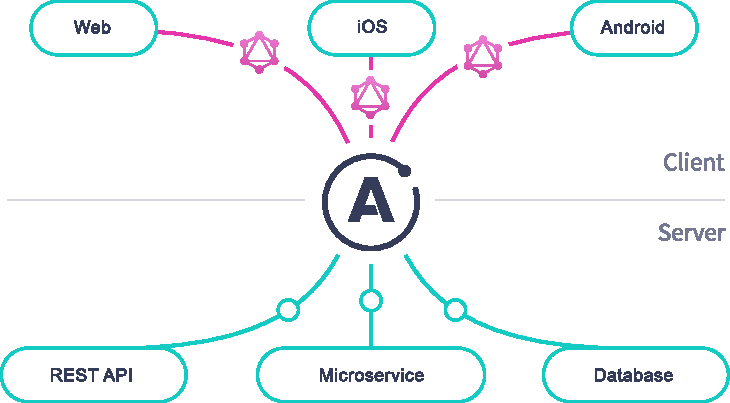
\includegraphics[scale=0.8]{obrazky-figures/apollo_server_diagram}
	\caption{Diagram architektúry Apollo Server. \cite{Apollo}}
\end{figure}

\noindent Apollo Server dokáže pôsobiť ako \emph{jednotná brána} pre všetky klientské aplikácie. Brána má predom definovanú schému, tzn. že klient presne vie aké operácie môže vykonávať a aké dáta môže očakávať späť.


